
We have developed a simple simulation tool to evaluate the model
that is publicly available from (URL removed for blind-review).
We omit the details of the simulation settings in this paper but all
the settings are described in the simulation tool.

%%\subsection{Simulation settings}

%%The simulation setting is shown in Figure~\ref{fig:topology-simple}.
%%\begin{itemize}
%%  \item		job: mean duration:4sec, mean 1 unit,
%%        frontend 1, backend 2 for data intensive job,
%%        frontend 2, backend 1 for interactive job,
%%  \item		node: capacity 100 for MDC, 1000 for DC
%%  \item		link: capacity 200 for MDC-DC, 1000 for DC-DC
%%\end{itemize}
%%
%%\begin{figure}[tb]
%%  \begin{center}
%%    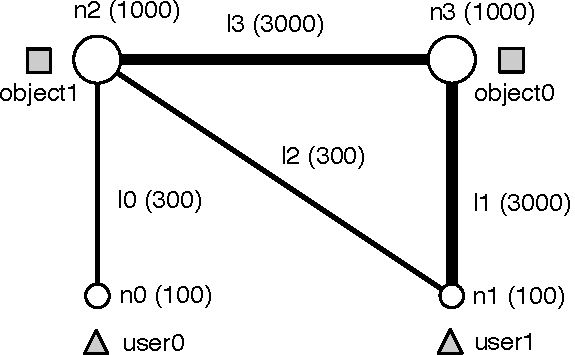
\includegraphics[width=7.5cm,clip]{topology-simple.pdf}
%%    \vspace{-2.0ex}
%%    \caption{simple simulation topology}
%%    \Description{Simulation topology with 2 datacenters and 2 micro datacenters.}
%%    \label{fig:topology-simple}
%%  \end{center}
%%\end{figure}
%%
%%Simulation scenarios:
%%\begin{enumerate}
%%  \item	{\bf node only:} 4 nodes without randomization to show how the
%%        cost function works
%%  \item	{\bf link only:} 4 links without randomization to show
%%        different costs affects
%%  \item	{\bf monotonic function:} same as above but use monotonic cost
%%        function.
%%  \item	{\bf randomize:} 4 nodes and 4 links with randomization
%%  \item {\bf comparison:} compared with, no idle-resource pooling
%%  \item	{\bf surge:} same as above but with a request surge at one location
%%  \item	{\bf edge computing:} 2 nodes (big and small) and 1 link, the
%%    users are closer to the small node. 2 types jobs (interactive,
%%    data intensive).  show interactive jobs are on the small node,
%%    data intensive jobs are on the big node.
%%  \item {\bf premium service:} 4 nodes with 3 standard and 1 premium services.
%%  \item	{\bf complex?:} realistic scenario
%%\end{enumerate}

\subsection{Basic Behaviors}

\begin{figure}[tb]
  \begin{center}
    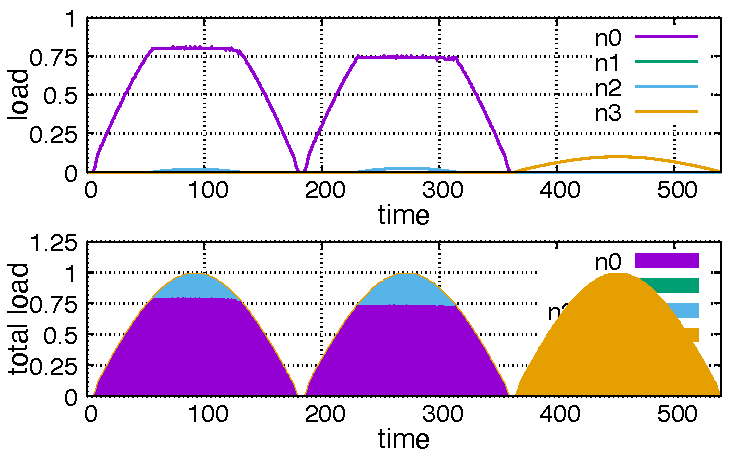
\includegraphics[width=1.0\columnwidth]{lowering.pdf}
    \vspace{-2.0ex}
    \caption{Cost manipulations: shifting the load +.2,
      +.4 and raising the weight for data access}
    \smallskip
    \raggedright
    \small
    Note that the capacity of DCs is 10 times larger than that of MDCs
    so that DC's load looks much smaller for the same volume of jobs.
    In the normalizede total load (bottom), the volume is normalized
    to the capacity $C$ of MDC to show the total volume of jobs:
    $\sum \tilde{\rho}$, \:$\tilde{\rho} = \rho \cdot C/C_{MDC}$.
    \Description{Simulation results to illustrate the effects of cost manipulations.}
    \label{fig:lowering}
  \end{center}
\end{figure}

The effects of manipulating the cost function and the resource weight
for a job is illustrated in Figure~\ref{fig:lowering}.
Here, a series of interactive jobs of the same type are generated in
4 waves between a user at MDC0 and an object at DC3 in
Figure~\ref{fig:system}.
In the first wave,  most of the jobs are assigned to the node closest
to the user (MDC0) but some overflowing jobs are offloaded to DC2.
The peak load of MDC0 is $.8$ in the first wave.
In the second and the third waves, the cost function of MDC0 is
manipulated to reduce the load by shifting the load by $.2$ and $.4$
respectively. As a result, the peak load of MDC0 is
reduced from $.8$ to $.6$ in the second wave, and then, to $.4$ in the
third wave.
In the fourth wave, the weight for the backend communication is
increased, and all jobs are assigned to the node that has the object
(DC3).

\subsection{Mixed Behaviors}

A more complex scenario is shown in Figure~\ref{fig:mixed}.
Again, the topology in Figure~\ref{fig:system} is used, and
random fluctuation is added to the interval and duration of jobs.
A series of jobs are generated
between user0 at MDC0 and an object at DC3, and
between user1 at MDC1 and an object at DC2.
Both have the ratio of $1:2$ for interactive vs. data-intensive jobs.
To observe offloading behaviors, user1's jobs are increased by a
factor of 2 in the third wave (time 360-540), and by a factor of 10 in
the fourth wave (time 540-720). 
Before time 360, interactive jobs are assigned closer to the users,
and data intensive jobs are assigned closer to the data.
In the third wave, MDC1 reaches the upper limit and overflowing jobs are
assigned to DC2.
In the fourth wave, the link MDC1-DC2 reaches the upper limit so that
overflowing jobs are assigned to DC3.
(To absorb the surge in the fourth wave in this scenario, enough
capacity is provided to the link MDC1-DC3.)
This scenario illustrates the responsive behavior of the system,
and how jobs for MDCs can be offloaded to upstream DCs.

\begin{figure}[tb]
  \begin{center}
    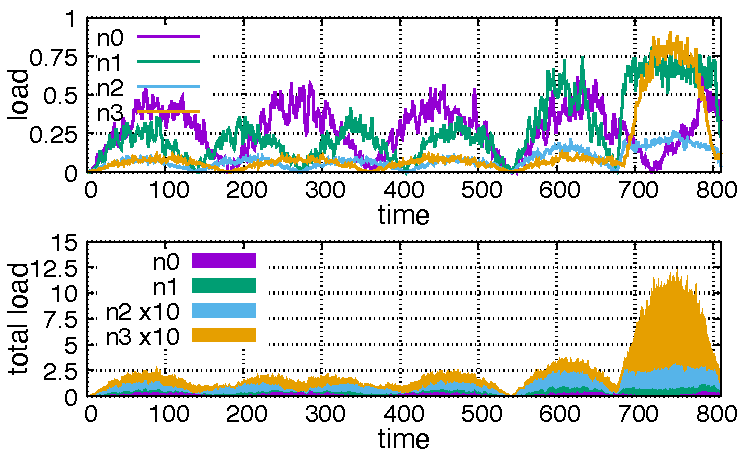
\includegraphics[width=1.0\columnwidth]{simu2.pdf}
    \vspace{-2.0ex}
    \caption{Mixed load with 2 DCs and 2 MDCs}
    \Description{Simulation results with mixed scenario.}
    \label{fig:mixed}
  \end{center}
\end{figure}

% \begin{figure}[tb]
%   \begin{center}
%     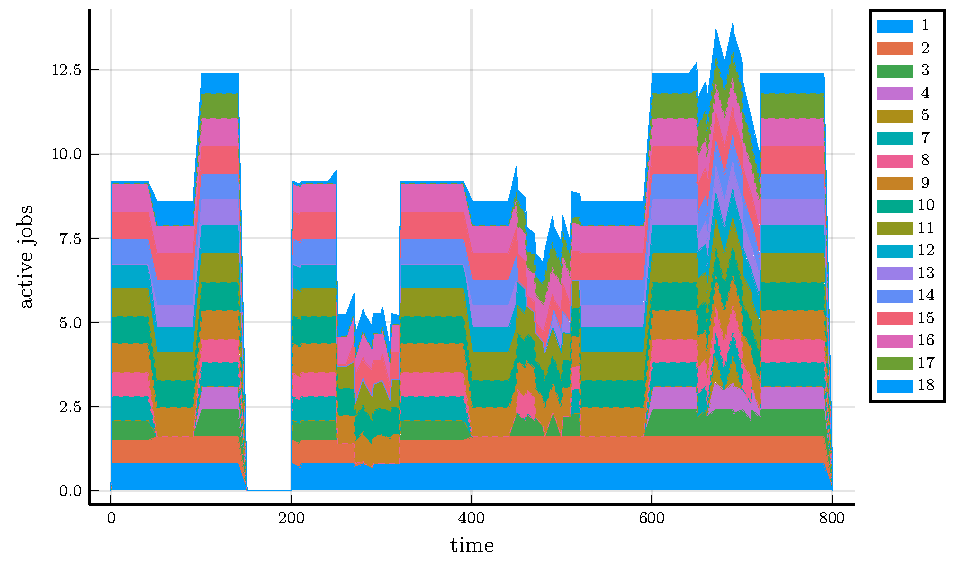
\includegraphics[width=1.0\columnwidth]{complex-convex-monotonic.pdf}
%     \vspace{-2.0ex}
%     \caption{Complex scenario with convex nodes and monotonic links}
%     \label{fig:complex}
%   \end{center}
% \end{figure}

% \begin{figure}[tb]
%   \begin{center}
%     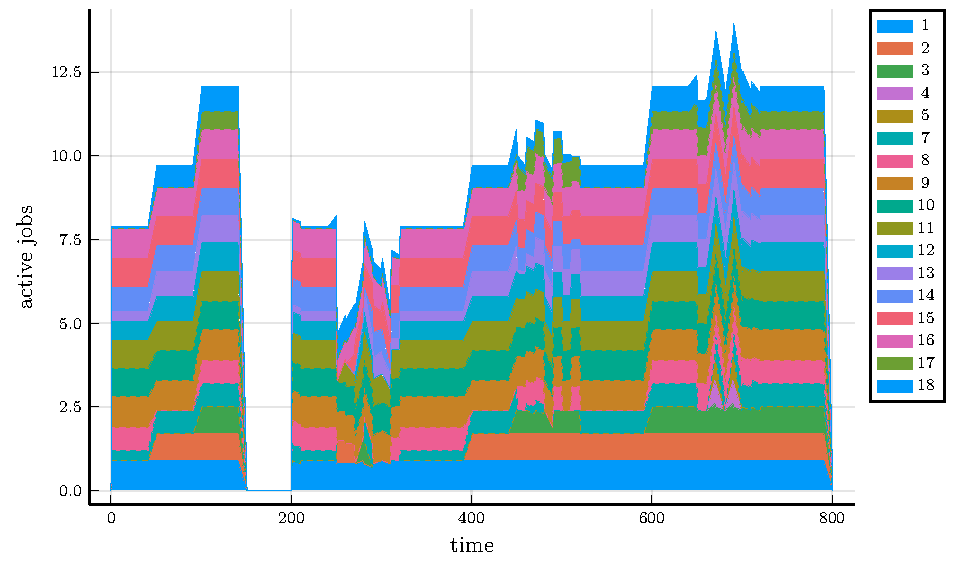
\includegraphics[width=1.0\columnwidth]{complex-full-convex.pdf}
%     \vspace{-2.0ex}
%     \caption{Complex scenario with convex nodes and monotonic links}
%     \label{fig:complex-convex}
%   \end{center}
% \end{figure}

% \begin{figure}[tb]
%   \begin{center}
%     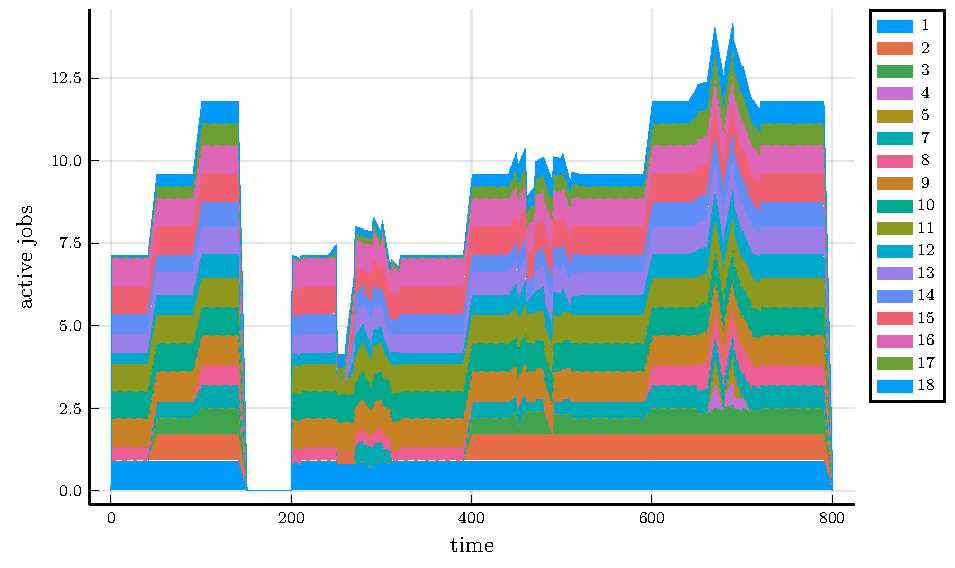
\includegraphics[width=1.0\columnwidth]{complex-full-monotonic.pdf}
%     \vspace{-2.0ex}
%     \caption{Complex scenario with convex nodes and monotonic links}
%     \label{fig:complex-monotonic}
%   \end{center}
% \end{figure}

\begin{figure}[tb]
  \centering
  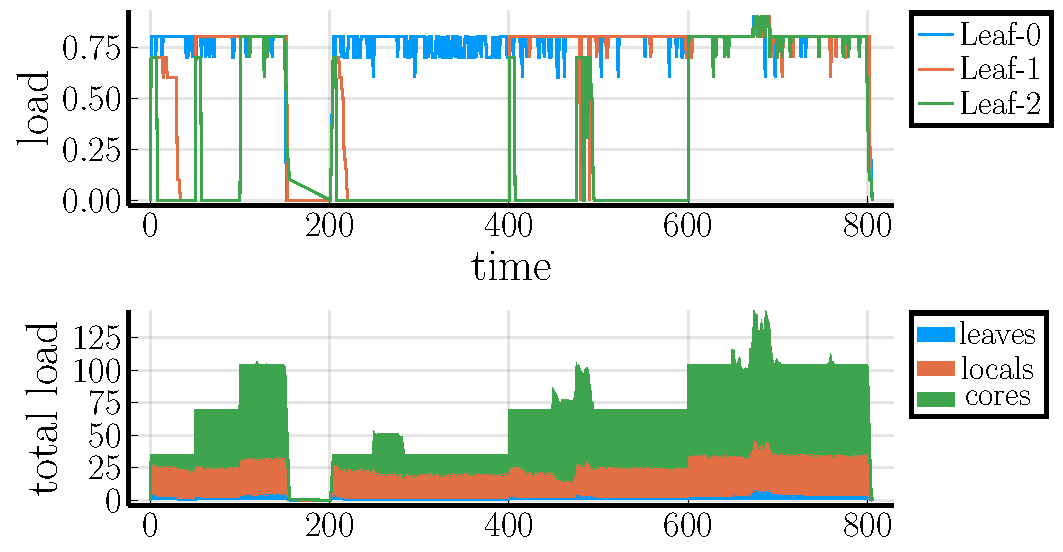
\includegraphics[width=\columnwidth]{18nodes.pdf}
  \vspace{-2.0ex}
  \caption{Mixed load with 18 DCs}
  \Description{A more complex scenario to illustrate offloading behaviors.}
  \label{fig:18nodes}
\end{figure}

The last scenario in Figure~\ref{fig:18nodes} shows a more complex case with
18 DCs: 2 cores, 8 locals and 8 leaves connected by a FAT-tree.
Each leaf-DC is connected to one local-DC, and a local-DC is connected to
2 core-DCs and 2 other local-DCs, or just to 2 other local-DCs.
Jobs are generated from all leaf-DCs and local-DCs.
The top plot shows the load of 3 leaf-DCs for readability.
We can see that the load stays at around $.75$ when a leaf-DC is
active, except during a short transient overshoot by a surge at time XX.
The results illustrate quick responses to changing load,
yet converging to stable states once the load is settled,
and offloading excess jobs to upstream data centers.

